% This file was created by matlab2tikz.
%
%The latest updates can be retrieved from
%  http://www.mathworks.com/matlabcentral/fileexchange/22022-matlab2tikz-matlab2tikz
%where you can also make suggestions and rate matlab2tikz.
%
\definecolor{mycolor1}{rgb}{0.85098,0.32549,0.09804}%
%
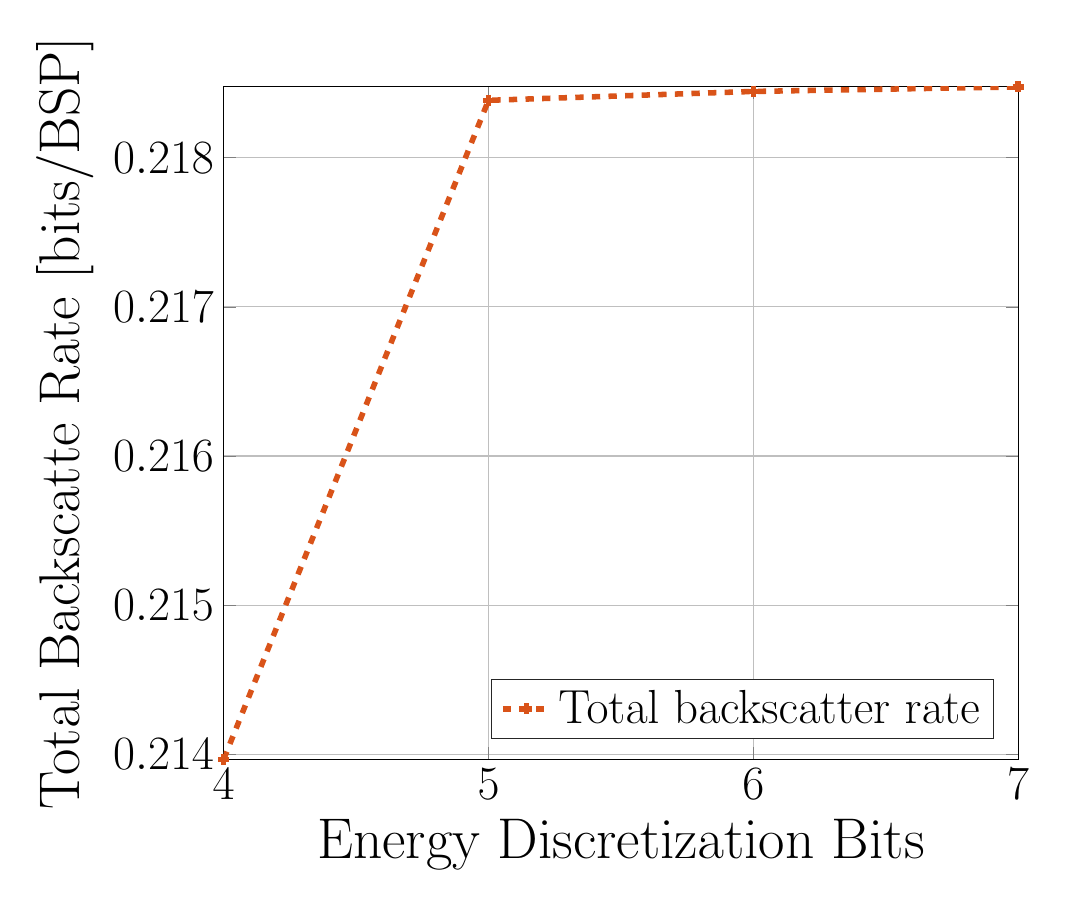
\begin{tikzpicture}

\begin{axis}[%
width=3.972in,
height=3.362in,
at={(0.666in,0.454in)},
scale only axis,
xmin=4,
xmax=7,
xtick={4, 5, 6, 7},
xlabel style={font=\color{white!15!black}},
xlabel={Energy Discretization Bits},
ymin=0.213966869419165,
ymax=0.218473997098467,
ylabel style={font=\color{white!15!black}},
ylabel={Total Backscatte Rate [bits/BSP]},
axis background/.style={fill=white},
xmajorgrids,
ymajorgrids,
legend style={at={(0.97,0.03)}, anchor=south east, legend cell align=left, align=left, draw=white!15!black},
title style={font=\huge},
label style={font=\huge},
ticklabel style={font=\LARGE},
legend style={font=\LARGE},
scaled y ticks=false,
y tick label style={/pgf/number format/.cd, fixed, precision=3}
]
\addplot [color=mycolor1, dashed, line width=2.0pt, mark=+, mark options={solid, mycolor1}]
  table[row sep=crcr]{%
4	0.213966869419165\\
5	0.218383940375522\\
6	0.218443547035828\\
7	0.218473997098467\\
};
\addlegendentry{Total backscatter rate}

\end{axis}
\end{tikzpicture}%